% ======================================================================
%  Section 4.7.3 --- Weight maps.  Replaces the empty heading on p.75.
%
%  FIGURES REQUIRED (two of the three already exist):
%    figures/gmap_v3_occluded_12.png   structure measure G, occluded, iter 12
%    figures/wmap_v3_occluded_12.png   Tukey weights,      occluded, iter 12
%    figures/wmap_v3_occluded_600.png  Tukey weights,      occluded, iter 600
%                                      <-- STILL TO PRODUCE: set the save
%                                      condition to iter == 2 || iter == 601
%
%  Section 4.6.4 currently promises weight maps for Variants 2 and 3. Only
%  Variant 3 produces them at present. Either add saveMaps() to Variant 2 or
%  amend 4.6.4 to promise Variant 3 alone. Variant 1 has D = I and its map is
%  uniformly white, so it should not be promised at all.
%
%  NOT CLAIMED HERE, DELIBERATELY: that the rejected region is the occluder
%  dilated by the filter support (Section 4.3.2). Measured on these maps the
%  rejected region is 2367 px against 4858 px for the flat region of G, i.e.
%  SMALLER, because the retained boundary rim eats into it and because the
%  weights are graded rather than binary. Establishing the dilation would
%  require measuring against the ellipse in the texture file itself, at a
%  stated weight threshold. Do not assert it from these figures.
% ======================================================================

\subsection{Weight maps}
\label{sec:weight-maps}

The quantitative results of Section~\ref{sec:ablation-results} establish that
the weighting recovers the pose under occlusion, but not that it does so for
the reason the method claims. The weights $w_j$ and the structure measure
$G(p)$ are both defined per measurement, so both can be displayed at their
image positions, and together they show the mechanism directly.

Figure~\ref{fig:maps-occluded} shows the two maps for Variant~3 at
iteration~12 of the occluded run. In the weight map, white denotes a retained
measurement, $w_j=1$, and black a rejected one, $w_j=0$; the ten-pixel border
that the filters cannot reach carries no measurement and is shown mid-grey so
that it is not mistaken for rejection. In the structure map, brightness is
proportional to $G(p)$, scaled so that three times the image mean saturates.

\paragraph{The occluder.}
In the structure map the occluding disc appears as a region of \emph{zero}
response, $G<0.02\,\bar{G}$ over a connected area of $4858$ pixels --- $7.4\%$
of the $66\,000$ measurements --- bounded by a bright rim that traces its
outline exactly. This is the behaviour required of a structure measure built
from first-order Gauss--Hermite kernels: the interior of the disc is uniform,
so its derivative response vanishes, while its boundary is a step edge and
produces the largest response in the image. The corresponding region of the
weight map is dark, and is likewise ringed by retained measurements.

The chain from~\eqref{eq:structG} to the control law is therefore visible end
to end. Inside the occluder $G$ vanishes, so $\bar{G}$ meets the floor
$\bar{G}_{\min}=0.1$ of~\eqref{eq:gbar}, the normalized residual
of~\eqref{eq:normalized-residual} is inflated tenfold, and the Tukey function
rejects it. On the boundary $G$ is maximal, the residual is reduced, and the
measurement is retained --- correctly, since the boundary of the occluder is
genuine image structure whose displacement does carry pose information.
Elsewhere $\bar{G}\approx1$ and the weighting is close to inert.

It is worth emphasising that this mechanism turns on the \emph{uniformity} of
the occluded region and not on its intensity. The structure measure adopted in
Section~\ref{sec:hermite-gate} has exactly zero DC gain, so a uniform bright
occluder would produce the same vanishing response and be rejected
identically. The limitation recorded in Section~\ref{sec:acknowledged} is
therefore the correct one to state, and is the only one: a \emph{textured}
occluder would produce a large $G$ and would not be suppressed by this
mechanism, whereas a uniform one is suppressed whatever its brightness.

\paragraph{Rejection away from the occluder.}
The maps also make visible an effect that Section~\ref{sec:tukey-limitation}
predicts but that the pose errors alone cannot show. At iteration~12 the mean
weight over the image is $0.75$, $4.2\%$ of measurements are rejected outright
and $16.0\%$ carry a weight below $0.25$. Since the occluder accounts for only
$7.4\%$ of the measurements, more than half of the strongly down-weighted
measurements lie outside it and are not corrupted at all. They are valid
measurements in photometrically sensitive regions whose residuals are
legitimately large because the misalignment is still gross, and which a
redescending estimator consequently rejects. This is the cost identified in
Section~\ref{sec:tukey-limitation}, quantified: early in the run the estimator
discards roughly twice as much information as the occlusion alone requires.

%%% FIGURE STILL TO PRODUCE --- see the header note. Once wmap at iteration
%%% 600 exists, this paragraph completes the argument; until then, delete it
%%% rather than describe a figure that does not exist.
Figure~\ref{fig:wmap-converged} shows the same map at iteration~600. The
scattered rejection has resolved and what remains is the occluder alone,
confirming that the effect above is transient and confined to the phase in
which the residual distribution has not yet contracted. The two panels
together bound the cost of robust weighting in time as well as in magnitude.

\begin{figure}[t]
    \centering
    \begin{subfigure}[b]{0.48\textwidth}
        \centering
        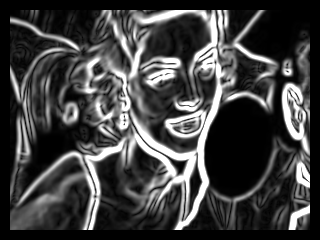
\includegraphics[width=\textwidth]{figures/gmap_v3_occluded_12.png}
        \caption{structure measure $G(p)$}
    \end{subfigure}
    \hfill
    \begin{subfigure}[b]{0.48\textwidth}
        \centering
        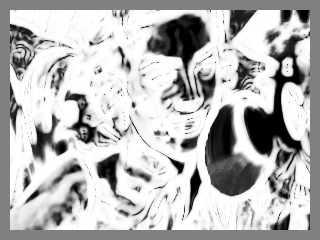
\includegraphics[width=\textwidth]{figures/wmap_v3_occluded_12.png}
        \caption{Tukey weights $w_j$}
    \end{subfigure}
    \caption{Variant~3 under occlusion, iteration~12. (a) The structure
    measure~\eqref{eq:structG}: the occluding disc gives a vanishing response
    over its uniform interior and the largest response in the image along its
    boundary. (b) The resulting weights: white retained, black rejected,
    mid-grey the filter border, which carries no measurement. The disc is
    rejected and its boundary retained.}
    \label{fig:maps-occluded}
\end{figure}

\begin{figure}[t]
    \centering
    \includegraphics[width=0.48\textwidth]{figures/wmap_v3_occluded_600.png}
    \caption{Variant~3 under occlusion, iteration~600. Compared with
    Figure~\ref{fig:maps-occluded}(b), the rejection scattered across the
    frame has resolved and only the occluder remains suppressed.}
    \label{fig:wmap-converged}
\end{figure}
